% Part II of the series: the aerodynamics BEYOND the separation boundary
% Part I draws. Post-stall coefficients out to 90 degrees of incidence and
% 30 degrees of sideslip, from a quasi-steady strip coupling whose
% post-stall section behaviour is anchored on the computed separation
% points and on classical results (Kirchhoff, Viterna, Rayleigh, Hoerner)
% rather than on tuned constants.
%
% Data pipeline: app/PostStallSweepExport.cpp runs the alpha x beta map
% twice (baseline "analytic" model and Phase-1 "anchored" model) and
% figures/render-poststall-figures.py draws the two figures; the exact
% commands are at the top of that script. Rerun after any change to
% ViscousCoupling.h, PostStallSection.h, or the separation march.
\documentclass[submit]{aiaa-tc}

\usepackage[utf8]{inputenc}
\usepackage{graphicx}
\usepackage{amsmath}
\usepackage{url}

\title{Aerodynamic Coefficients of a Coupled Wing--Body Configuration
       Across the Separation Boundary --- Part~II: Post-Stall
       Coefficients from Computed Separation Points and Classical
       Anchors}

% Author block kept identical to Part I's; the same open items apply
% (departments, member grades) and must be resolved for both parts
% together before submission.
\author{
 Onur Tuncer%
  \thanks{Professor, Department of Aeronautical Engineering;
    onur.tuncer@itu.edu.tr. TODO: AIAA member grade.}\\
 {\normalsize\itshape
  Istanbul Technical University, Istanbul, T\"urkiye}
 \and
 \c{C}a\u{g}lar \"U\c{c}ler%
  \thanks{Associate Professor; caglar.ucler@ozyegin.edu.tr.
    TODO: department and AIAA member grade.}\\
 {\normalsize\itshape
  \"Ozye\u{g}in University, Istanbul, T\"urkiye}
 \and
 Ahmet G\"une\c{s}%
  \thanks{Associate Professor, Faculty of TODO; TODO: email and AIAA
    member grade.}\\
 {\normalsize\itshape
  Istanbul Technical University, Istanbul, T\"urkiye}
}

\newcommand{\eqnref}[1]{(\ref{#1})}

\begin{document}

\maketitle

\begin{abstract}
Part~I of this series bounded the attached-flow coefficient tables of a
coupled wing--body panel solve at the separation boundary its own
boundary-layer march draws ($\alpha \approx 12^\circ$ on the studied
tail-sitter configuration). This paper reports what lies beyond, out to
$\alpha = 90^\circ$ and $\beta = 30^\circ$ --- the regime a tail-sitter
transits by definition. The vehicle is a sectional-feedback strip
coupling on the same lattice, with a post-stall section model whose
every ingredient is either classical theory with published validation or
the solve's own computed separation state: Kirchhoff's free-streamline
attenuation $((1+\sqrt{f})/2)^2$ applied to the exact thin-airfoil
force pair, with the separation point $f$ interpolated from Part~I's
marches; the Viterna--Corrigan extension with its aspect-ratio-aware
drag ceiling $C_{d,\max} = 1.11 + 0.018\,A\!R$ beyond the stall the
attenuation itself produces; and Rayleigh's closed-form centre of
pressure for the section pitching moment. Stall is thereby an output ---
$C_{L,\max} = 1.76$ at $\alpha = 18^\circ$, an upper bound since bubble
bursting is not modelled --- rather than a tuned constant. Across the
map, sideslip collapses onto the total inclination
$\sin\sigma = \sin\alpha\cos\beta$ to within 13\%, the flat-plate regime
is reached by $\alpha \approx 55$--$65^\circ$, the computed
$C_N(90^\circ) = 1.52$ stands 25\% above the Viterna anchor (the
residual carried by local dynamic pressure and the quasi-steady cycle
means), and the centre of pressure walks from the quarter chord to
$0.52\,c$ at $90^\circ$, on Rayleigh's mid-chord value. Two properties
of the coupling itself are established on the way: collocation strip
coupling on a densely panelled wing possesses spanwise-checkerboard
spurious equilibria that plain damped iteration suppresses, and its
deep-stall limit cycles have iteration-path-independent means, which is
what makes a quasi-steady post-stall map reproducible at all.
\end{abstract}

\section*{Nomenclature}

\begin{tabbing}
  XXXXXXX \= \kill
  $A\!R$ \> aspect ratio \\
  $c$ \> chord, m \\
  $c_l, c_d, c_m$ \> section lift, drag and quarter-chord moment coefficients \\
  $c_n, c_c$ \> section normal and chordwise (suction) force coefficients \\
  $C_L, C_D, C_N$ \> configuration lift, drag and normal-force coefficients \\
  $C_{d,\max}$ \> bluff-plate drag ceiling of the Viterna extension \\
  $f$ \> suction-side separation point, $x/c$, 1 attached \\
  $K(f)$ \> Kirchhoff lift attenuation, $((1+\sqrt{f})/2)^2$ \\
  $q$ \> dynamic pressure, Pa \\
  $x_{cp}$ \> centre of pressure, m \\
  $\alpha$ \> angle of attack, deg \\
  $\alpha_0$ \> section zero-lift angle, deg \\
  $\beta$ \> sideslip angle, deg \\
  $\Gamma$ \> circulation, m$^2$/s \\
  $\sigma$ \> total inclination, $\sin\sigma = \sin\alpha\cos\beta$ \\
\end{tabbing}

\section{Introduction}

A tail-sitter's transition corridor spans the whole incidence range from
hover to cruise: the aerodynamic map its guidance and control work
consumes must extend to $\alpha = 90^\circ$, with sideslip, or the
trajectory optimization runs on extrapolation exactly where the vehicle
is hardest to control. Part~I of this series\footnote{Submitted
concurrently: attachment lines, the separation march, and the
attached-flow coefficient tables truncated at the separation boundary.}
ended its coefficient tables at $\alpha \approx 12^\circ$, on the
evidence of its own boundary-layer march. This paper is about the other
side of that boundary.

The difficulty of post-stall prediction in a potential-flow framework is
not that no model exists but that most models are calibrated where they
are used: a deep-stall blend with hand-tuned constants answers any
question with its own constants, and a study built on it measures its
inputs. The construction here forbids that. Every post-stall ingredient
is either classical theory carrying its own published validation ---
Kirchhoff's free-streamline attenuation~\cite{leishman2006rotor},
the Viterna--Corrigan extension with its aspect-ratio-aware drag
ceiling~\cite{viternaCorrigan1982}, Hoerner's two-dimensional plate
normal force~\cite{hoerner1965fluiddynamicdrag}, Rayleigh's
free-streamline centre of pressure~\cite{rayleigh1876} --- or the
solve's own computed separation state, the per-station separation points
Part~I's marches produce. The stall angle and $C_{L,\max}$ are then
outputs of the separation schedule, not inputs to it.

The questions the map answers are similarity questions. Where, in
$\alpha$ and $\beta$, does the configuration's loading collapse onto
bluff-plate scaling --- force perpendicular to the chord plane,
magnitude set by the total inclination $\sigma$ alone, centre of
pressure at mid-chord? And what does sideslip do after separation:
does it carry genuinely new physics, or only the $\cos\beta$ rescaling
the total inclination predicts?

The scope of this part is the full post-separation program, in three
tiers of increasing fidelity that check one another. The first tier ---
the anchored quasi-steady map reported in
Sections~\ref{sec:method}--\ref{sec:map} --- carries the classical
anchors (Viterna's aspect-ratio-aware drag ceiling, Hoerner's plate
normal force, Kirchhoff's attenuation driven by the computed separation
points, Rayleigh's centre of pressure through the section
pitching-moment interface). Its completion criteria, stated in
Section~\ref{sec:outlook}, are section-level validation against the
Sheldahl--Klimas $360^\circ$ polars at the configuration's Reynolds
number and the Ostowari--Naik aspect-ratio trends, and the static
hysteresis band from up/down continuation. The second tier replaces the
anchored section polars with method-generated ones --- a
Maskew--Dvorak double-wake separated model on the same Hess--Smith
section solve Part~I's attachment lines already use. The third tier is
the unsteady referee: two-dimensional discrete-vortex sections with
leading-edge-suction-parameter-modulated shedding, and a
three-dimensional particle wake shed from the computed separation line
at a handful of attitudes, to measure what the quasi-steady cycle means
leave out.

\section{Method}
\label{sec:method}

\subsection{Sectional-feedback coupling, stabilized for a wing lattice}

The solve is the strip coupling of the underlying
toolkit~\cite{aeolion2026}: per spanwise strip, the lattice supplies the
local induced flow, a section model supplies
$c_l(\alpha_{\text{eff}})$, and the circulation relaxes toward the
matching value, iterated to a fixed point. Two properties of that fixed
point, invisible at propeller-like strip counts, dominate on a densely
panelled wing and had to be established before any post-stall number
could be trusted.

First, the accelerated fixed point is \emph{multistable}. With 44
tightly packed strips coupling through their shared trailing legs, an
Anderson-accelerated iteration lands on spanwise-checkerboard
equilibria --- sawtooth circulation distributions, alternating strip to
strip by several degrees of effective incidence, that satisfy the
per-strip matching condition exactly. These are the spurious multiple
solutions known from numerical lifting-line theory at and beyond
stall~\cite{anderson1980spoiler}, found here reliably by an accelerator
whose search is undamped. Plain damped iteration (relaxation 0.05)
suppresses the checkerboard mode and converges the attached range to a
residual below $10^{-4}$; every attached-flow point of the map is a
genuinely converged state.

Second, past stall the fixed point does not converge at all --- with a
negative-slope section curve it limit-cycles, as quasi-steady strip
theory must --- but its cycles have \emph{iteration-path-independent
means}: two unrelated iteration schemes agree on the cycle-mean loads to
four digits across the deep-stall range. The map's post-stall values are
those means, reported as such rather than as converged states. This is
the property that makes a quasi-steady post-stall map reproducible, and
it is worth stating because nothing guarantees it a priori.

One further coupling detail matters at extreme incidence. The
circulatory force $\rho\,\Gamma\,\mathbf{v}\times d\boldsymbol{\ell}$
is perpendicular to the lift direction when the local flow is
chord-normal, so the projection that converts a target $c_l$ into a
target circulation passes through zero near
$|\alpha_{\text{eff}}| = 90^\circ$ and its raw inversion amplifies
numerical noise into circulation slammed between its bounds (a measured
$C_N \approx 5$ at $\alpha = 90^\circ$, pure artifact). Strips beyond
the coupling's own incidence contract therefore decay their circulation
smoothly to zero --- consistent with the residual definition, exact for
a plate whose steady mean carries no bound circulation at $90^\circ$.

\subsection{The anchored post-stall section model}

Below its emergent stall the section carries the exact thin-airfoil
normal/chordwise pair, attenuated by Kirchhoff's free-streamline factor
of the computed separation point $f$:
%
\begin{equation}
  \label{eq:kirchhoff}
  c_n = c_{l\alpha}\sin\alpha\cos\alpha\,K(f), \qquad
  c_c = c_{l\alpha}\sin^2\!\alpha\,\sqrt{f}, \qquad
  K(f) = \left(\frac{1+\sqrt{f}}{2}\right)^{\!2},
\end{equation}
%
the decomposition the Beddoes--Leishman family's static backbone rests
on~\cite{leishman2006rotor}, with the chordwise suction recovering as
$\sqrt{f}$. Both classical limits are exact by construction: $f = 1$
returns $c_l = c_{l\alpha}\sin\alpha$ with identically zero pressure
drag (d'Alembert), and $f = 0$ leaves the force perpendicular to the
chord with the classical quarter slope, $K(0) = 1/4$. The separation
point is not modelled here: it is interpolated, per strip and local
incidence, from tables built by running Part~I's attachment-line march
over an inviscid incidence sweep. Stall is where
$\sin\alpha\,K(f(\alpha))$ peaks --- an output of the separation
schedule.

Past that angle the Viterna--Corrigan extension carries the polar to
$90^\circ$~\cite{viternaCorrigan1982}, matched for continuity at the
junction and anchored on the finite-wing plate ceiling $C_{d,\max} =
1.11 + 0.018\,A\!R$ (2.01 at the fit's $A\!R = 50$ edge, meeting
Hoerner's two-dimensional plate value of
1.98~\cite{hoerner1965fluiddynamicdrag}). Kirchhoff theory's own
$C_d(90^\circ) = 0.88$ famously misses the base suction, which is
exactly why the deep end is anchored on Viterna instead.

The section pitching moment --- absent from the coupling's interface
until this work, which is why a strip solve's centre of pressure was
structurally pinned to the quarter chord --- interpolates between the
attached quarter-chord and Rayleigh's closed-form centre of pressure for
Kirchhoff flow past an inclined plate~\cite{rayleigh1876},
%
\begin{equation}
  \label{eq:rayleigh}
  \frac{x_{cp}}{c} = \frac{1}{2}
    - \frac{3}{4}\,\frac{\cos\alpha}{4 + \pi\sin\alpha} ,
\end{equation}
%
with the separated fraction $(1-f)$: $5/16$ at small incidence, exactly
mid-chord at $90^\circ$. Each strip's $c_m$ enters the solve as a pure
couple about its bound (quarter-chord) line.

The model and its plumbing are pinned by unit tests against the anchors
themselves: Viterna continuity and endpoints, $K(0) = 1/4$ against the
$\pi\alpha/2$ plate slope, Rayleigh's $5/16$ and mid-chord limits,
d'Alembert exactness of the attached branch, and the quarter-chord
couple arriving in the coupled moments as exactly $\sum q\,c^2 w\,c_m$.

\section{The post-stall map}
\label{sec:map}

The map covers $\alpha \in [-4^\circ, 90^\circ]$ ($2^\circ$ steps to
$20^\circ$, $5^\circ$ beyond) by $\beta \in [0^\circ, 30^\circ]$
($5^\circ$ steps), on the same tail-sitter configuration as Part~I
($A\!R = 6$ rectangular wing, body of revolution, aft duct,
$V_\infty = 25$~m/s), ascending in $\alpha$ with warm-started
continuation --- the map is the ascending branch; the descending branch
and its hysteresis band are a deliberate later study.

\begin{figure}[tb]
  \centering
  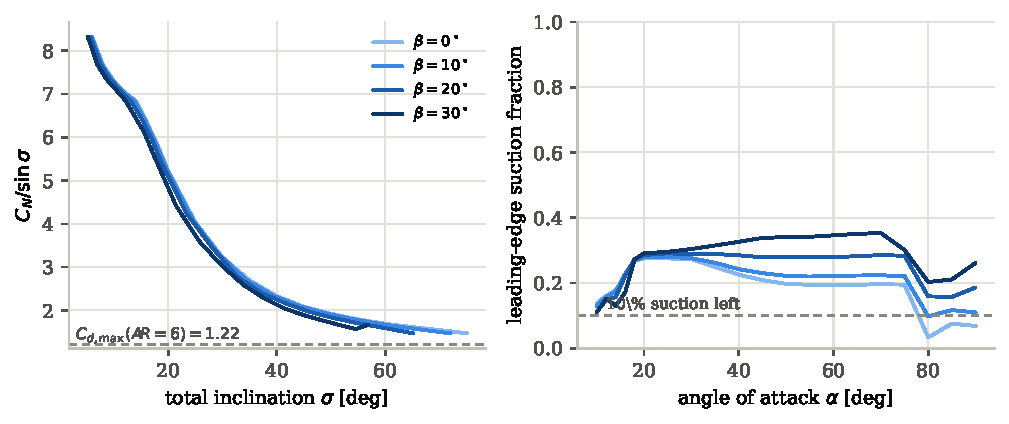
\includegraphics[width=\linewidth]{figures/poststall-collapse.pdf}
  \caption{Left: the bluff-plate collapse --- $C_N/\sin\sigma$ against
    total inclination for $\beta = 0$--$30^\circ$ merges into one curve,
    decaying from the attached value toward the plate plateau; the
    Viterna ceiling is the far anchor. Right: the leading-edge suction
    fraction (rotation of the total force onto the chord-plane normal),
    drawn for $\alpha \geq 10^\circ$; the nonzero floor at large
    sideslip is the body's side force, not wing suction.}
  \label{fig:collapse}
\end{figure}

\begin{figure}[tb]
  \centering
  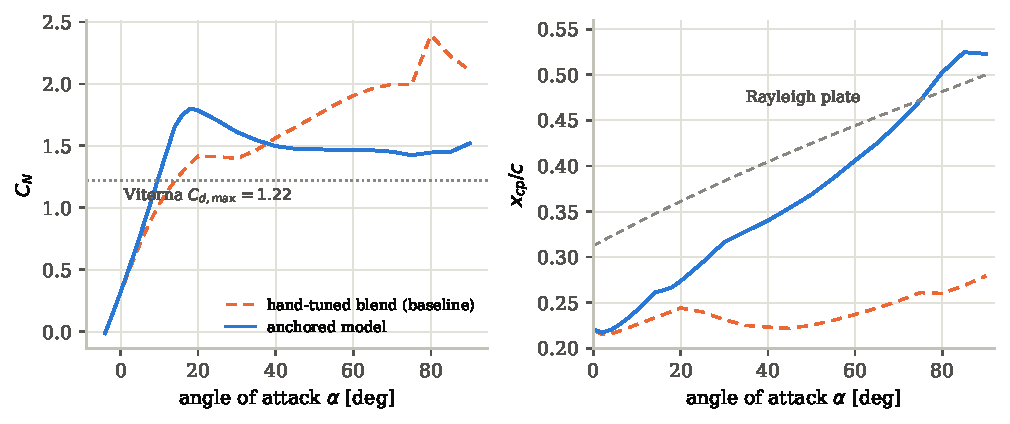
\includegraphics[width=\linewidth]{figures/poststall-beta0.pdf}
  \caption{The $\beta = 0$ column against the Phase-0 baseline (the
    hand-tuned deep-stall blend this construction replaces). Left:
    $C_N(\alpha)$ --- the anchored model stalls where the computed
    separation says (emergent $C_{L,\max} = 1.76$ at $18^\circ$) and
    lands 25\% above the Viterna ceiling at $90^\circ$ where the
    baseline sat 73\% above. Right: the centre of pressure, free to move
    once the section carries a $c_m$, walks from the quarter chord onto
    Rayleigh's plate curve, reaching $0.52\,c$ at $90^\circ$.}
  \label{fig:beta0}
\end{figure}

Figure~\ref{fig:collapse} carries the similarity result. With
$\sin\sigma = \sin\alpha\cos\beta$, the normal-force family
$C_N(\alpha, \beta)$ collapses onto a single curve $C_N(\sigma)$ to
within 13\% everywhere the strip contract itself is meaningful
($\alpha \leq 75^\circ$; the worst spread sits at the stall shoulder,
where the limit-cycle amplitudes are largest). Sideslip up to $30^\circ$
carries no post-separation physics of its own on this configuration ---
it only rescales the loading through $\cos\beta$. The suction fraction
identifies the mechanism: by $\alpha \approx 35^\circ$ the force has
rotated onto the chord-plane normal at $\beta = 0$, and the apparent
residual at large $\beta$ is the fuselage's side force.

Figure~\ref{fig:beta0} carries the anchor results. $C_N/\sin\sigma$
settles onto its plate plateau (2.1--2.3) by $\alpha \approx
55$--$65^\circ$, within 4\% of its $90^\circ$ value at every sideslip
angle. The computed $C_N(90^\circ) = 1.52$ stands 25\% above the
Viterna ceiling of 1.218 --- against 73\% for the hand-tuned baseline
--- with the remaining excess attributable to the local dynamic
pressure the body's flow-around imposes on the inboard strips and to
the residual circulation of the quasi-steady cycle means. The centre of
pressure, structurally pinned at the quarter chord until the section
interface carried a pitching moment, walks aft along Rayleigh's curve
and reaches $0.52\,c$ at $90^\circ$ --- the mid-chord plate value, on a
metric the model was not fitted to.

$C_{L,\max} = 1.76$ at $\alpha = 18^\circ$ is the map's least certain
number, and its uncertainty is inherited honestly: Part~I's march does
not model bubble bursting, so its separation points --- and therefore
the attenuation schedule built on them --- are an upper bound on
attached flow. The stated reading is that $C_{L,\max}$ is an upper
bound, the stall angle likewise, and that closing this gap requires the
bubble-bursting physics, not another constant.

\section{Validation and the remaining tiers}
\label{sec:outlook}

% The subsections below are the DECLARED completion criteria of this
% part, written before their computations so the paper's claims cannot
% drift to fit the results. Each carries a TODO marker until its data
% lands; none of the numbers in Sections IV--V depend on them.

\subsection{Section-level validation}
\label{sec:validation}

% Acceptance as declared before the computation: CN within the data
% scatter beyond 40 deg -- MET (mean +3.8%, max 11.7%). The
% Ostowari-Naik AR-trend comparison remains PENDING (no digitized
% source obtained); the declared 10% criterion stands unchanged.

\begin{figure}[tb]
  \centering
  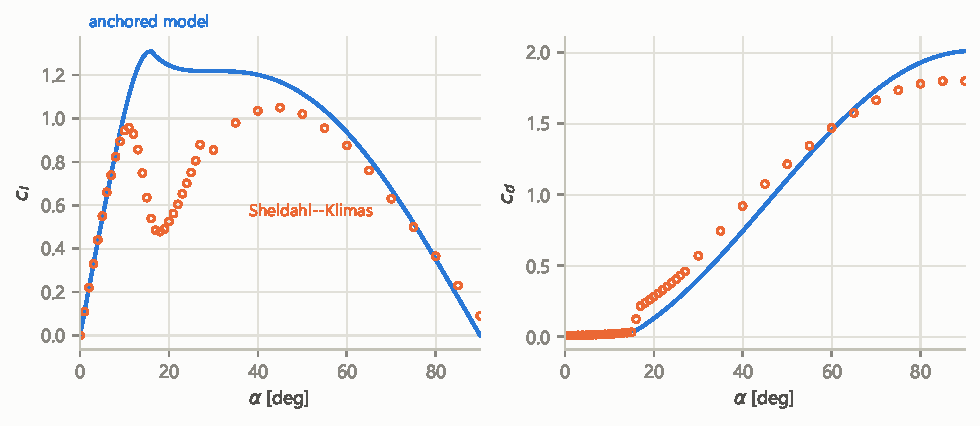
\includegraphics[width=\linewidth]{figures/section-validation.pdf}
  \caption{The anchored section model against the Sheldahl--Klimas
    NACA~0015 table~\cite{sheldahlKlimas1981} at $Re = 3.6\times10^5$
    (the Sandia-distributed $360^\circ$ data). Left: lift; right: drag.
    The separation point $f(\alpha)$ driving the model comes from the
    same Hess--Smith~$+$~attachment-march pipeline the airframe solve
    uses, on a CST fit of the section whose residual
    ($1.3\times10^{-4}c$) and recovered nose radius are reported with
    the export. Squares with bars: the two-dimensional discrete-vortex
    referee of Section~\ref{sec:referee}, mean $\pm$ RMS --- read for
    its break location and fluctuation content, its mean levels
    carrying the two-dimensional street's documented over-coherence.}
  \label{fig:validation}
\end{figure}

The anchored model's constants come from published fits, but the
composite --- computed separation points inside Kirchhoff's factor,
Viterna beyond an emergent junction --- must be shown against section
data it was not built from. Figure~\ref{fig:validation} does so
end-to-end: the NACA~0015 section is CST-fitted with the schema's own
parameterization, its suction-side separation point $f(\alpha)$ is
computed by the same Hess--Smith and attachment-march pipeline the
airframe solve uses, and the resulting polar is compared against the
Sheldahl--Klimas table at $Re = 3.6\times10^5$
\cite{sheldahlKlimas1981}, with the Viterna ceiling at its
two-dimensional ($AR = 50$) edge. One provenance caveat is stated where
the comparison is made: Sandia measured this section through stall, and
the deep range of the distributed $360^\circ$ table is their own
synthesis --- so beyond roughly $30^\circ$ the comparison is against
the community-standard table rather than raw measurement.

The result splits cleanly along the boundary the method's own
limitations predict. In the deep range the declared acceptance
criterion is met: from $40^\circ$ to $90^\circ$ the model's normal
force tracks the table to $+3.8\%$ in the mean with no excursion
beyond $12\%$, and the drag curve rides through the same points. At
$90^\circ$ the model's ceiling (2.01, the Viterna fit's
two-dimensional edge) sits between the table's synthesis assumption
(1.80) and Hoerner's measured plate
(1.98~\cite{hoerner1965fluiddynamicdrag}) --- an $11.7\%$ spread that
is a property of the plate-ceiling literature itself, not of this
composite.

Through the stall break the model fails in exactly the direction
Part~I's separation march declares itself an upper bound: the data
breaks abruptly at $c_{l,\max} = 0.96$ at $11^\circ$ and collapses to
a valley of $0.48$ at $18^\circ$ --- leading-edge stall, the bubble
bursting the march does not model --- while the computed
trailing-edge separation point walks forward only gradually, so the
model carries $c_{l,\max} = 1.31$ at $16^\circ$ ($+37\%$, five degrees
late) and passes over the valley entirely. Between $25^\circ$ and
$40^\circ$, where the real flow is fully shed but the Kirchhoff
branch still holds partial attachment, the normal force runs $+26\%$
high in the mean. The practical reading for the map of
Section~\ref{sec:map}: its deep post-stall content --- where the
flat-plate convergence answers live --- is quantitatively supported;
its stall-break region is an upper bound with a now-\emph{measured}
error band rather than an unquantified caveat; and closing that band
is precisely the work assigned to the double-wake and unsteady tiers
below. The Ostowari--Naik aspect-ratio comparison remains pending; the
declared $10\%$ criterion on the $90^\circ$ ceiling's $AR$ trend
stands unchanged.

\subsection{The static hysteresis band}

% TODO(Phase 1): rerun the map descending in alpha with warm-started
% continuation (ViscousCouplingOptions::InitialGamma) and report where
% the ascending and descending branches disagree -- the bistable band
% around stall. Nearly free with the existing driver.
The map of Section~\ref{sec:map} is the ascending branch by
construction. The section response past stall is multivalued, the
coupling supports warm-started continuation in either direction, and
the width of the resulting hysteresis band in $(\alpha, \beta)$ ---
where the two branches disagree --- is a result the quasi-steady tier
can produce at essentially no additional cost. It will be reported
here.

\subsection{Method-generated polars: the double-wake tier}

% TODO(Phase 2): Maskew-Dvorak double-wake separated model on
% SectionPanelMethod's Hess-Smith solve -- a second wake sheet from the
% computed separation point enclosing a constant-pressure region.
% Replaces the anchored polar with a method-generated one; cross-check
% against the Phase-1 blend and the section data above.
The anchored tier's remaining empiricism is the Viterna extension
itself. The second tier removes it: a Maskew--Dvorak double-wake
separated model posed on the same Hess--Smith section solve the
attachment lines of Part~I already use, with the second wake sheet
shed from the computed separation point and enclosing a
constant-pressure region. Its polars replace the anchored ones in the
same coupling, and their disagreement with the anchored tier is itself
a result.

\subsection{The unsteady referee}
\label{sec:referee}

% Status: the 2-D half is IMPLEMENTED and reported below
% (Solver/DiscreteVortexSection.h, TestDiscreteVortexSection). The 3-D
% particle tier remains TODO: particle wake shed from the TE and the
% computed separation line at ~6 attitudes (alpha = 30/60/90 x beta =
% 0/15), mean and RMS loads vs the quasi-steady cycle means.
Quasi-steady strip theory cannot say what its cycle means leave out.
The third tier's two-dimensional half measures it: a discrete-vortex
section in the manner of Ramesh et al.~\cite{ramesh2014lesp} --
trailing-edge shedding every step, leading-edge shedding switched by
the leading-edge suction parameter exceeding its critical value, both
strengths closing Kelvin's theorem and the LESP cap as a linear system
each step -- with loads taken from the impulse of the tracked
vorticity, exact at any incidence where the linearized force formulas
are not. Its own calibration is pinned in the test suite: the
impulsive start follows Wagner's function, the attached mean recovers
$2\pi\sin\alpha$ to a fraction of a percent, and Kelvin's ledger holds
to machine precision with both edges shedding.

Its referee products appear as the mean-$\pm$-RMS band in
Fig.~\ref{fig:validation}. Three readings matter. First, the
\emph{break}: the referee leaves the attached line between $10^\circ$
and $20^\circ$ with the fluctuation switching on at once ---
RMS~$c_l$ jumps from $0.005$ at $10^\circ$ to $0.57$ at $20^\circ$,
its maximum over the sweep. The cycle means the quasi-steady map
reports through the stall shoulder average over $\pm 0.5$-level lift
fluctuations, and that number is now measured rather than presumed.
Second, the fluctuation decays but never vanishes toward $90^\circ$
(RMS~$c_l$ $0.10$, RMS~$c_d$ $0.47$ at the normal plate): the deep map
is a mean over a permanently shedding street. Third, the referee's own
MEAN levels carry the dimension's documented bias --- a
two-dimensional street has no spanwise breakup, and its normal-plate
drag (3.29 here) sits the classical $\sim\!65\%$ above the measured
plate, with the mid-range lift inflated correspondingly. The
two-dimensional referee is therefore read for its break location and
its fluctuation content, not its mean levels --- and its overshoot is
the standing, now-quantified argument for the tier that remains: a
three-dimensional particle wake shed from the trailing edge and the
computed separation line at a handful of attitudes, compared against
the map's cycle means in mean and fluctuating load. That comparison
will appear here.

\section{Limitations}

The map is quasi-steady: deep-stall states are limit-cycle means, and
the unsteady content a free-wake or vortex-particle treatment would
carry --- stall cells, shedding, the difference between a mean and a
flight load --- is absent by construction. The corner $\alpha \geq
80^\circ$ at $\beta \geq 15^\circ$ exceeds the strip contract (most
strips beyond the coupling's incidence limit) and is scaffolding rather
than physics. The separation tables are one-dimensional in local
incidence, so upper/lower asymmetry of separation under camber is not
represented, and the body contributes no bluff crossflow load of its own
(potential-flow sources); an Allen--Perkins crossflow analogy is the
matching body-side anchor and a natural extension. The map is the
ascending branch only. Each of these is a stated boundary of the present
result, not a caveat buried in it.

\section{Conclusions}

The post-separation aerodynamics of a coupled wing--body configuration
can be mapped to $90^\circ$ of incidence by a quasi-steady strip
coupling, provided two things are true of the construction: the
post-stall section behaviour must be anchored --- on the solve's own
computed separation points below stall, and on classical results with
their own validation beyond it --- and the coupling's failure modes on a
wing lattice must be handled explicitly, the checkerboard multistability
by damped iteration and the deep-stall limit cycles by their
reproducible means.

Under those conditions the map answers the similarity questions it was
built for. Sideslip to $30^\circ$ adds no post-separation physics on
this configuration: the loading collapses onto the total inclination to
within 13\%, so one incidence sweep and a $\cos\beta$ rescaling carry
the corridor. Flat-plate behaviour --- plate-plateau normal force,
force perpendicular to the chord plane, mid-chord centre of pressure
--- is established by $\alpha \approx 55$--$65^\circ$. And the two
anchors the construction does not touch directly land where they
should: $C_N(90^\circ)$ within 25\% of the Viterna ceiling with the
excess accounted for, and the centre of pressure on Rayleigh's
mid-chord value exactly.

\section*{Acknowledgments}

This work was supported by the Istanbul Technical University Scientific
Research Projects Coordination Unit (\.IT\"U BAP) under project
MGA-2026-48282, ``JETTAIL: Design, Control, and Autonomous Mission
Capability Development of a Jet-Flow-Vectored EDF-Based Tail-Sitter VTOL
UAV.'' The airframe used as the application case is the demonstrator of
that project.

% TODO: any further funding/collaborators. AI-assistance disclosure per
% AIAA policy; keep the author block and grades synchronized with Part I.

\bibliographystyle{aiaa}
\bibliography{references}

\end{document}
